\documentclass[12pt]{article}
\usepackage[utf8]{inputenc}
\usepackage[T1]{fontenc}
\usepackage{amsmath}
\usepackage{amsfonts}
\usepackage{amssymb}
\usepackage[version=4]{mhchem}
\usepackage{stmaryrd}
\usepackage{bbold}
\usepackage{graphicx}
\usepackage[export]{adjustbox}
\graphicspath{ {./images/} }

\title{Assignment 4: Simulations with MPS }


\author{Instructor: Lesik Motrunich\\
TA: Liam O'Brien}
\date{}


%New command to display footnote whose markers will always be hidden
\let\svthefootnote\thefootnote
\newcommand\blfootnotetext[1]{%
  \let\thefootnote\relax\footnote{#1}%
  \addtocounter{footnote}{-1}%
  \let\thefootnote\svthefootnote%
}

%Overriding the \footnotetext command to hide the marker if its value is `0`
\let\svfootnotetext\footnotetext
\renewcommand\footnotetext[2][?]{%
  \if\relax#1\relax%
    \ifnum\value{footnote}=0\blfootnotetext{#2}\else\svfootnotetext{#2}\fi%
  \else%
    \if?#1\ifnum\value{footnote}=0\blfootnotetext{#2}\else\svfootnotetext{#2}\fi%
    \else\svfootnotetext[#1]{#2}\fi%
  \fi
}

\begin{document}
\maketitle
Due: $4 \mathrm{pm}$ Thursday, May 28,2024

\section*{1 Introduction to modern applications of MPS}
In this assignment, we will finally be able to use matrix product states (MPS) to study systems larger than can be handled with exact diagonalization, by employing techniques that are currently being used in condensed matter research. As we can no longer make reference to an exact wavefunction, typically we will begin with some trial variational ansatz in the form of an MPS and perform an optimization or some other protocol to produce a quantum state of interest. In principle this introduces additional complexity, as well as problems of interpretation, to our solutions that were not present in ED. However, what we gain by surpassing the system-size limitations of exact diagonalization far outweighs these costs. It turns out that this new paradigm of tensor networkbased methods can eventually take us beyond the realm of many-body physics in one dimension, and in fact many of the interesting results that are currently being produced in condensed matter physics using these techniques are studies of higher-dimensional systems.

The seminal tensor network numerical method is the density matrix renormalization group (DMRG), introduced by Steve White in 1992, although it actually preceded our understanding of MPS. Here we will study another protocol which has the benefit of a very clear intuitive picture and, like DMRG, currently enjoys widespread usage. This is time-evolving block decimation (TEBD)-

invented by Guifre Vidal at Caltech in 2004 - in which the unitary time-evolution operator $e^{-i t H}$ under some Hamiltonian $H$ is decomposed into a particular pattern of "gate" operations which implement a map on the space of MPS. TEBD has a particularly useful versatility, in that with only minor changes it can produce either "cooling" to the ground state under imaginary time evolution, or quantum dynamics under real time evolution. We will explore both applications, studying the benefits and drawbacks for classical simulations of quantum systems.

\section*{2 Gauging MPS}
One of the technical considerations arising from the MPS ansatz is a gauge freedom in the definition of the virtual indices. Suppose we have an MPS


\begin{equation*}
|\psi\rangle=\sum_{\boldsymbol{\sigma}} \sum_{a_{1}, a_{2}, \ldots, a_{L-1}}\left(A^{1}\right)_{a_{1}}^{\sigma_{1}}\left(A^{2}\right)_{a_{1}, a_{2}}^{\sigma_{2}} \cdots\left(A^{L}\right)_{a_{L-1}}^{\sigma_{L}}|\boldsymbol{\sigma}\rangle \tag{1}
\end{equation*}


Between any tensors on adjacent sites we can insert an identity matrix acting on the virtual degree of freedom. The identity can be expanded into $\mathbb{I}=X^{-1} X$ for some invertible matrix $X$ :


\begin{align*}
\sum_{a_{j}}\left(A^{j}\right)_{a_{j-1}, a_{j}}^{\sigma_{j}}\left(A^{j+1}\right)_{a_{j}, a_{j+1}}^{\sigma_{j+1}} & =\sum_{a_{j}, a_{j}^{\prime}}\left(A^{j}\right)_{a_{j-1}, a_{j}}^{\sigma_{j}} \mathbb{I}_{a_{j}, a_{j}^{j}}\left(A^{j+1}\right)_{a_{j}^{\prime}, a_{j+1}}^{\sigma_{j+1}} \\
& =\sum_{a_{j}, a_{j}, \tilde{a}_{j}}\left(A^{j}\right)_{a_{j-1}, a_{j}}^{\sigma_{j}}\left(X^{-1}\right)_{a_{j}, \tilde{a}_{j}} X_{\tilde{a}_{j}, a_{j}^{\prime}}\left(A^{j+1}\right)_{a_{j}^{\prime}, a_{j+1}}^{\sigma_{j+1}} \\
& =\sum_{\tilde{a}_{j}}\left(\left(A^{j}\right)^{\sigma_{j}} X^{-1}\right)_{a_{j-1}, \tilde{a}_{j}}\left(X\left(A^{j+1}\right)^{\sigma_{j+1}}\right)_{\tilde{a}_{j}, a_{j+1}} \\
& \equiv \sum_{\tilde{a}_{j}}\left(\tilde{A}^{j}\right)_{a_{j-1}, \tilde{a}_{j}}^{\sigma_{j}}\left(\tilde{A}^{j+1}\right)_{\tilde{a}_{j}, a_{j+1}}^{\sigma_{j+1}} . \tag{2}
\end{align*}


That is, the virtual degrees of freedom may be transformed in this way under any invertible matrix, and physical observables will be unaffected because the tensor contractions yield the same outcomes. This makes more precise the idea that the actual numbers stored in MPS tensors are usually not informative by themselves. We say that individual tensor components are not gauge invariant: instead of being indicative of physics by themselves, they are a byproduct of the scheme we happen to be using.

\subsection*{2.1 Canonical forms}
We should try to exploit gauge invariance by making a particularly convenient choice of gauge. It will become evident that certain choices can drastically reduce the difficulty of specific calculations; these particular gauge choices are collectively referred to as MPS canonical forms.

Consider the problem of compressing an ED wavefunction into an MPS, which we did in Assignment 2. After performing an SVD between the first site and the rest of the system, we write the state in the following matricized form:


\begin{equation*}
C_{\sigma_{1},\left(\sigma_{2}, \ldots, \sigma_{L}\right)}=\sum_{a_{1}} U_{\sigma_{1}, a_{1}} S_{a_{1}, a_{1}}\left(V^{\dagger}\right)_{a_{1},\left(\sigma_{2}, \ldots, \sigma_{L}\right)} \tag{3}
\end{equation*}


where $U$ and $V$ satisfy the orthogonality condition $U^{\dagger} U=\mathbb{I}, V^{\dagger} V=\mathbb{I}$. Using the relabeling $A^{1} \equiv U$ and explicitly writing the indices, this condition becomes for the MPS tensor


\begin{equation*}
\sum_{\sigma_{1}}\left(A^{1 \dagger}\right)_{a_{1}^{\prime}, \sigma_{1}}\left(A^{1}\right)_{\sigma_{1}, a_{1}}=\mathbb{I}_{a_{1}^{\prime}, a_{1}}=\delta_{a_{1}^{\prime}, a_{1}} \tag{4}
\end{equation*}


That is, the summation over the physical index leads to a trivial identification of the virtual indices (here $a_{j}^{\prime}$ is the same index as $a_{j}$, but differentiated by coming from the conjugated state). If we continue, creating the MPS by setting $A^{j} \equiv U$ and contracting $S$ and $V^{\dagger}$ at each step, each subsequent MPS tensor-excepting the last-satisfies an orthogonality condition of the form


\begin{equation*}
\sum_{\sigma_{j}, a_{j-1}}\left(A^{j \dagger}\right)_{a_{j}^{\prime},\left(a_{j-1}, \sigma_{j}\right)}\left(A^{j}\right)_{\left(a_{j-1}, \sigma_{j}\right), a_{j}}=\delta_{a_{j}^{\prime}, a_{j}}, j=2, \ldots, L-1 \tag{5}
\end{equation*}


Now consider computing the squared norm $\langle\psi \mid \psi\rangle$ of the MPS. Remember that when writing the MPS initially, we "reshaped" the tensor, writing the matrix $\left(A^{j}\right)_{\left(a_{j-1}, \sigma_{j}\right), a_{j}}$ as $\left(A^{j}\right)_{a_{j-1}, a_{j}}^{\sigma_{j}}$. For example, the left-orthogonality condition above reads $\sum_{a_{j-1}, \sigma_{j}}\left(\left(A^{j}\right)_{a_{j-1}, a_{j}^{\sigma_{j}}}^{\sigma_{j}}\right)^{*}\left(A^{j}\right)_{a_{j-1}, a_{j}}^{\sigma_{j}}=\delta_{a_{j}^{\prime}, a_{j}}$, or in matrix form $\sum_{\sigma_{j}}\left(\left(A^{j}\right)^{\sigma_{j}}\right)^{\dagger}\left(A^{j}\right)^{\sigma_{j}}=\mathbb{I}$. At each step we can use the orthogonality conditions (4) and (5) to eliminate pairs of tensors and their Hermitian conjugates:

$$
\begin{aligned}
& \langle\psi \mid \psi\rangle=\sum_{\substack{a_{1}, a_{2}, \ldots, a_{L-1} \\
a_{1}^{\prime}, a_{2}^{2}, \ldots, a_{L-1}^{-}}} \sum_{\sigma_{1}, \ldots, \sigma_{L}}\left(\left(A^{1}\right)_{a_{1}^{\prime}}^{\sigma_{1}} *^{*}\left(\left(A^{2}\right)_{a_{1}^{1}, a_{2}^{\prime}}^{\sigma_{2}}\right)^{*} \cdots\left(\left(A^{L}\right)_{a_{L-1}}^{\sigma_{L}}\right)^{*}\left(A^{1}\right)_{a_{1}}^{\sigma_{1}}\left(A^{2}\right)_{a_{1}, a_{2}}^{\sigma_{2}} \cdots\left(A^{L}\right)_{a_{L-1}}^{\sigma_{L}}\right.
\end{aligned}
$$

\begin{center}
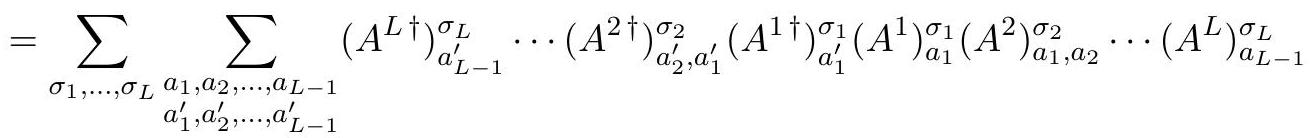
\includegraphics[max width=\textwidth]{2024_05_17_c251ec82fd3768475949g-03(1)}
\end{center}

\begin{center}
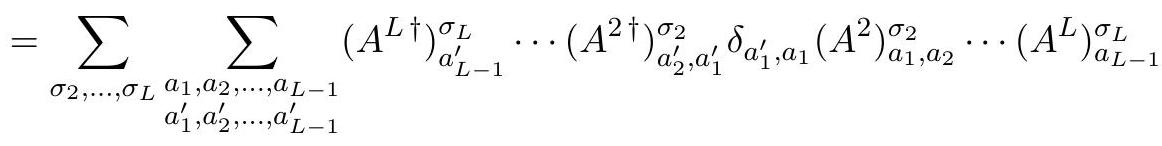
\includegraphics[max width=\textwidth]{2024_05_17_c251ec82fd3768475949g-03}
\end{center}


\begin{align*}
& =\sum_{\substack{\sigma_{2}, \ldots, \sigma_{L}}} \sum_{\substack{a_{1}, a_{2}, \ldots, a_{L-1} \\
a_{2}^{\prime}, \ldots, a_{L-1}^{L}}}\left(A^{L \dagger}\right)_{a_{L-1}^{L}}^{\sigma_{L}} \cdots\left(A^{3 \dagger}\right)_{a_{3}^{3}, a_{2}^{\prime}}^{\sigma_{3}^{\prime}}\left(A^{2}\right)_{a_{2}^{2}, a_{1}}^{\dagger \sigma_{2}}\left(A^{2}\right)_{a_{1}, a_{2}}^{\sigma_{2}}\left(A^{3}\right)_{a_{2}, a_{3}}^{\sigma_{3}} \cdots\left(A^{L}\right)_{a_{L-1}}^{\sigma_{L}} \\
& =\sum_{\sigma_{3}, \ldots, \sigma_{L}} \sum_{\substack{a_{2}, \ldots, a_{L-1}^{\prime} \\
a_{2}^{\prime}, \ldots, a_{L-1}^{\prime}}}\left(A^{L \dagger}\right)_{a_{L-1}^{L}}^{\sigma_{L}} \cdots\left(A^{3 \dagger}\right)_{a_{3}^{3}, a_{2}^{\prime}}^{\sigma_{3}} \delta_{a_{2}^{\prime}, a_{2}}\left(A^{3}\right)_{a_{2}, a_{3}}^{\sigma_{3}} \cdots\left(A^{L}\right)_{a_{L-1}}^{\sigma_{L}} \\
& \vdots \\
& =\sum_{\sigma_{L}} \sum_{a_{L-1}}\left(A^{L \dagger}\right)_{a_{L-1}}^{\sigma_{L}}\left(A^{L}\right)_{a_{L-1}}^{\sigma_{L}} \\
& =\sum_{\sigma_{L}} \sum_{a_{L-1}} V_{\sigma_{L}, a_{L-1}} S^{2}\left(V^{\dagger}\right)_{a_{L-1}, \sigma_{L}} \\
& =S^{2} \tag{6}
\end{align*}


Recalling that $S$ is diagonal, we reproduce the criterion that the state is normalized if its squared Schmidt values sum to unity (here, for the cut between sites $L-1$ and $L$ ). This calculation is far more compactly represented in the tensor network graphical language. The orthogonality condition (5) for the tensors is shown in Fig. 1, and the full contraction (6p) in Fig. 2.

Crucially, despite the unwieldiness of the first line in (6), we did almost no actual work to perform this calculation. The orthogonality rule allowed nearly every tensor contraction to be replaced by a delta function, the only exception being on site $L$. This is a result of the gauge choice we made in generating the SVD: by making the tensors "left-orthogonal" we put the MPS in what is known as left canonical form. In such a canonical form we refer to the single site (here, $j=L$ ) whose tensor contracts nontrivially as the orthogonality center.

If we had tried to contract the network from the right, beginning at site $L$, we would have been unable to use the orthogonality condition and would have needed to compute every contraction manually, and obtained the same result. However, it is easy to imagine running the MPS creation process the other way, starting with site $L$ and working to the left, now relabeling $A^{j} \equiv V^{\dagger}$ at every step. Then we could contract from the right using the "right-orthogonality" of the $V^{\dagger}$ matrices. In this case the orthogonality center is site 1 , and the MPS is in right canonical form.

\begin{center}
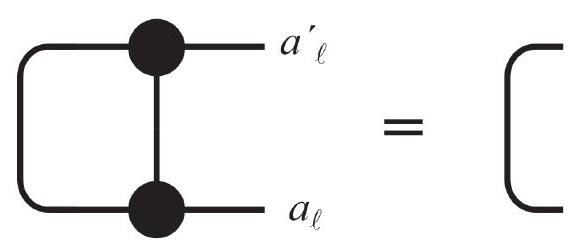
\includegraphics[max width=\textwidth]{2024_05_17_c251ec82fd3768475949g-04}
\end{center}

Figure 1: The left-orthogonality condition (5) for MPS tensor $A^{\ell}$, in tensor network notation. In the graphical notation, the connection of two indices without a tensor represents a delta function.

\begin{center}
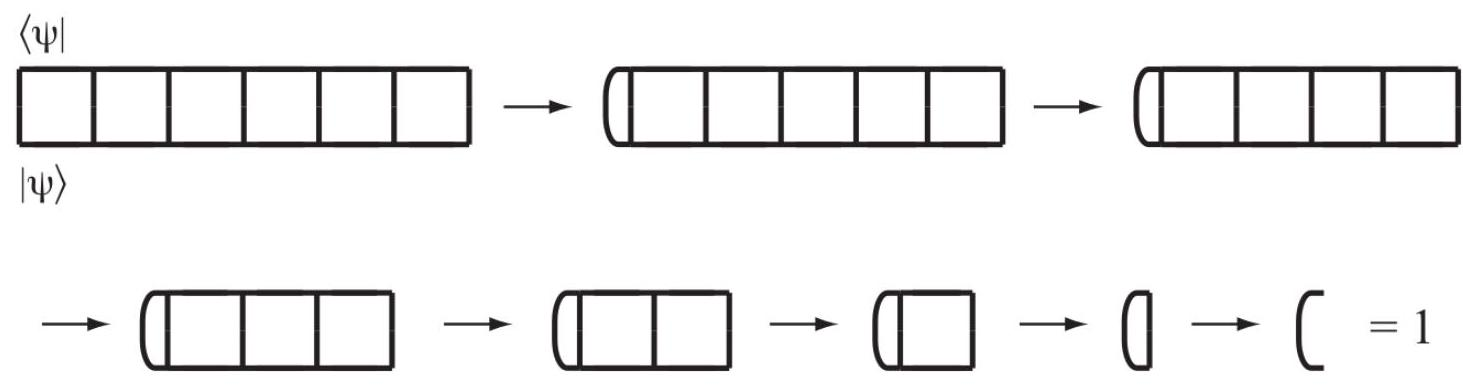
\includegraphics[max width=\textwidth]{2024_05_17_c251ec82fd3768475949g-04(1)}
\end{center}

Figure 2: Tensor network for the squared norm (6), where tensors are not explicitly drawn but are implicitly placed at all intersections of more than 2 legs, and at sharp corners. The first step uses (4) and all subsequent steps use (5), illustrated in Fig. 1. Here the state is already normalized.

\subsection*{2.2 Choosing a gauge for calculations}
Let us generalize the calculation of the squared norm in the previous section to find the expectation value of a local observable in the state $|\psi\rangle$. Suppose we have a left-canonical MPS and wish to measure a single-site operator $O_{j}=\sum_{\sigma_{j}, \sigma_{j}^{\prime}} \sigma^{\sigma_{j}^{\prime}, \sigma_{j}}\left|\sigma_{j}^{\prime}\right\rangle\left\langle\sigma_{j}\right|$ acting on the site $j=L$. As we have seen, this looks very similar to the tensor network for the overlap, but with $O_{L}$ sandwiched vertically between $\langle\psi|$ and $|\psi\rangle$ on site $L$, indicative of an operation on the physical index $\sigma_{L}$. The expression for this quantity is identical to that of $\langle\psi \mid \psi\rangle$ except on the last site; thus, orthogonality allows us to reduce the contraction immediately to


\begin{equation*}
\left\langle O_{L}\right\rangle=\sum_{\sigma_{L}, \sigma_{L}^{\prime}, a_{L-1}}\left(A^{L \dagger}\right)_{a_{L-1}}^{\sigma_{L}^{\prime}}\left(O_{L}\right)^{\sigma_{L}^{\prime}, \sigma_{L}}\left(A^{L}\right)_{a_{L-1}}^{\sigma_{L}} \tag{7}
\end{equation*}


This measurement is independent of system size! A serendipitous choice of gauge allows us to compute local observables at site $L$ with effort that is constant in the number of sites. It is evident that right canonical gauge allows the same for observables at site 1.

In fact, the above are special cases and generically we can specify a mixed canonical form with orthogonality center at site $j$. Begin with, say, an MPS in right canonical form, so for $j>1$ the tensors satisfy $\sum_{\sigma_{j}, a_{j}}\left(A^{j}\right)_{a_{j-1}, a_{j}}^{\sigma_{j}}\left(A^{j \dagger}\right)_{a_{j}, a_{j-1}^{\prime}}^{\sigma_{j}}=\delta_{a_{j-1}, a_{j-1}^{\prime}}$. The orthogonality center can be moved from site 1 to site 2 as follows. Contract $\sum_{a_{1}}\left(A^{1}\right)_{a_{1}}^{\sigma_{1}}\left(A^{2}\right)_{a_{1}, a_{2}}^{\sigma_{2}}=W_{a_{2}}^{\sigma_{1}, \sigma_{2}}$, then perform an SVD (on the appropriately reshaped $W$; the reshaping is clear from the indices):


\begin{equation*}
W_{\sigma_{1},\left(\sigma_{2}, a_{2}\right)}=\sum_{\tilde{a}_{1}} U_{\sigma_{1}, \tilde{a}_{1}} S_{\tilde{a}_{1}, \tilde{a}_{1}}\left(V^{\dagger}\right)_{\tilde{a}_{1},\left(\sigma_{2}, a_{2}\right)}=\sum_{\tilde{a}_{1}}\left(\tilde{A}^{1}\right)_{\tilde{a}_{1}}^{\sigma_{1}}\left(\tilde{A}^{2}\right)_{\tilde{a}_{1}, a_{2}}^{\sigma_{2}} \tag{8}
\end{equation*}


with $\tilde{A^{1}} \equiv U$ and $\tilde{A^{2}} \equiv S V^{\dagger}$. Now $\tilde{A}^{1}$ is left orthogonal, and as we have not touched $A^{3}, A^{4}, \ldots, A^{L}$, they remain right-orthogonal. The orthogonality center is at site 2 , and accordingly $\tilde{A}^{2}$ itself is\\
neither left- nor right-orthogonal. Now the tensor network for measuring $\left\langle O_{2}\right\rangle$ looks like the one shown in Fig. 3, which uses both orthogonality conditions.

The above simplification of measurements is not the only benefit to using MPS canonical forms: in practice, they also provide the crucial benefit of allowing consistent truncation of a quantum state. In order to utilize the compression afforded by MPS, we of course need the ability to truncate Schmidt values across a cut. We could always just contract two MPS tensors and perform an SVD, eliminating some low-weight contributions, but generally the singular values of this matrix will not coincide with the Schmidt values of the quantum state. However, for an MPS in canonical form it turns out that the SVD at the orthogonality center does indeed correspond to the Schmidt decomposition of the entire state. This can easily be seen using the orthogonality rules. In practice, accurate truncation of a virtual index requires that one works at an orthogonality center, in order to use the true Schmidt values of the MPS.

\begin{center}

\includegraphics[max width=\textwidth]{2024_05_17_c251ec82fd3768475949g-05}
\end{center}

Figure 3: The tensor network for measuring a single-site observable at the orthogonality center has the same structure regardless of the system size.

\section*{3 TEBD algorithm}
The underlying idea behind TEBD is simple: in order to time-evolve a quantum state, we wish to apply the operator $U(t)=e^{-i t H}$ to some initial MPS representation. However it is not clear that this can be accomplished efficiently: the computational savings achieved by MPS rely on locality and $U(t)$ is certainly a nonlocal operator. The solution is to not apply $U(t)$ to the state, but rather a controlled approximation to $U(t)$ which relies on the locality of the Hamiltonian and the Trotter expansion for matrix exponentials. This allows for time evolution, and, by rotating to imaginary time $\tau=i t$, we may also approximate the thermal operator $e^{-\tau H}$, which for large $\tau$ "cools" a state by increasing its overlap with the ground state of $H$ (provided the state has nonzero overlap initially). This works very much like the power method described in Assignment 1, where $e^{-\tau H}$ can be thought of as its Taylor expansion.

\subsection*{3.1 Trotter decomposition}
The Hamiltonian itself is of course not a general Hermitian operator but a sum of local terms. We cannot quite use this fact to compute the exponential naively because unless all terms commute, the exponential of their sum is not the same as the product of the separate exponentials. This is expressed in the Zassenhaus formula


\begin{equation*}
e^{t(A+B)}=e^{t A} e^{t B} e^{-t^{2}[A, B] / 2} \cdots \tag{9}
\end{equation*}


where factors not shown are higher order in $t$ [this formula is easily checked by Taylor-expanding both sides keeping terms to $O\left(t^{2}\right)$ ]. By minimizing the exponent of the $O\left(t^{2}\right)$ and higher factors,\\
these become very close to unity and to a good approximation we are in fact able to replace $e^{t(A+B)}$ with $e^{t A} e^{t B}$. To be more precise,


\begin{equation*}
e^{t(A+B)}=\lim _{n \rightarrow \infty}\left(e^{t A / n} e^{t B / n}\right)^{n} \tag{10}
\end{equation*}


This describes breaking up $t$ into $n$ pieces, each with factor $t / n$ in the exponent, all of which are multiplied together. In this way we can make the approximation arbitrarily close to the true matrix exponential by increasing $n$. The Suzuki-Trotter decomposition is based on using (10) to make a controlled approximation for $U(t)$ for Hamiltonians.

Consider an arbitrary 2-local Hamiltonian: $H=\sum_{j} h_{j, j+1}$, where the $h_{j, j+1}$ are 2-site operators. This is a very common class of models in quantum many-body physics. We can make the connection to Suzuki-Trotter explicit by grouping terms in $H$ based on the parity of $j$; that is, $H=H_{\text {even }}+H_{\text {odd }}$, where $H_{\text {even }}=\sum_{j=2,4,6, \ldots} h_{j, j+1}$ and $H_{\mathrm{odd}}=\sum_{j=1,3,5 \ldots \ldots} h_{j, j+1}$. Then within each grouping all terms commute, so in the language of the Trotter formula (10), we can approximate time evolution as


\begin{equation*}
|\psi(t)\rangle=e^{-i t H}\left|\psi_{0}\right\rangle=e^{-i t\left(H_{\text {even }}+H_{\text {odd }}\right)}\left|\psi_{0}\right\rangle \approx\left(\prod_{j \text { even }} e^{-i t h_{j, j+1} / n} \prod_{j \text { odd }} e^{-i t h_{j, j+1} / n}\right)^{n}\left|\psi_{0}\right\rangle \tag{11}
\end{equation*}


for large $n$. Each of the unitary operators $e^{-i t h_{j, j+1} / n}$ is referred to as a "Trotter gate," and is perturbatively close (in $1 / n$ ) to the identity. The nonlocal time-evolution operator $U(t)$ is replaced by $n$ rounds of acting with all of the Trotter gates in this particular grouping, each evolving the state by $\Delta t=t / n$. Importantly, the collection of Trotter gates maintains the locality of the original Hamiltonian, allowing us to use the efficiency afforded by MPS.

\subsection*{3.2 Application of gates to MPS}
The implementation of the Trotter decomposition for MPS is the foundation of TEBD. We continue with the 2-local Hamiltonian $H=\sum_{j} h_{j, j+1}=H_{\text {even }}+H_{\text {odd }}$, and will first apply the Trotter gates for the terms in $H_{\text {odd }}$; these are illustrated in Fig. 4 for an 8 -site system.

The application of a 2-local Trotter gate should restore the MPS form at the end, in order to be iterable. Consider applying the Trotter gate


\begin{equation*}
T=e^{-i t h_{j, j+1}}=\sum_{\substack{\sigma_{j}, \sigma_{j+1} \\ \sigma_{j}^{\prime}, \sigma_{j+1}^{\prime}}} T_{\sigma_{j}^{j}, \sigma_{j+1}^{\prime}}^{\sigma_{j}, \sigma_{j+1}}\left|\sigma_{j}, \sigma_{j+1}\right\rangle\left\langle\sigma_{j}^{\prime}, \sigma_{j+1}^{\prime}\right| \tag{12}
\end{equation*}


to sites $j$ and $j+1$ of an MPS. The steps are as follows. First, note that we added a prime to the upward-pointing physical indices of the MPS, as they will be summed over in the contraction. Contract both physical indices and the virtual index of the MPS:


\begin{equation*}
W_{a_{j-1}, a_{j+1}}^{\sigma_{j}, \sigma_{j+1}}=\sum_{\sigma_{j}^{\prime}, \sigma_{j+1}^{\prime}, a_{j}}\left(A^{j}\right)_{a_{j-1}, a_{j}}^{\sigma_{j}^{\prime}} T_{\sigma_{j}^{\prime}, \sigma_{j+1}^{\prime}}^{\sigma_{j}, \sigma_{j+1}^{\prime}}\left(A^{j+1}\right)_{a_{j}, a_{j+1}}^{\sigma_{j+1}^{\prime}} \tag{13}
\end{equation*}


Now $W$ represents the action of the gate on the two sites, but we aren't done because it's only a single tensor representing more than one physical degree of freedom. To regain the MPS form

we compute the SVD: $W_{\left(a_{j-1}, \sigma_{j}\right),\left(\sigma_{j+1}, a_{j+1}\right)}=\sum_{\tilde{a}_{j}} U_{\left(a_{j-1}, \sigma_{j}\right), \tilde{a}_{j}} S_{\tilde{a}_{j}, \tilde{a}_{j}}\left(V^{\dagger}\right)_{\tilde{a}_{j},\left(\sigma_{j+1}, a_{j+1}\right)}$. Note that the dimension of $\tilde{a}_{j}$ may exceed our desired bound $\chi$ on the bond dimension. This is unavoidable; we cannot enforce the bound on the bond dimension until applying all Trotter gates arising from the time evolution operator $U(t)$. That is, we must apply the full term inside the parentheses in

(11) before truncating. Now we can choose how to assign the MPS tensors after the SVD, either combining $\tilde{A}^{j} \equiv U S$ and $\tilde{A}^{j+1} \equiv V^{\dagger}$, or instead $\tilde{A}^{j} \equiv U$ and $\tilde{A}^{j+1} \equiv S V^{\dagger}$. Because in general we will not be performing the operation at the orthogonality center, both choices break the canonical form. (Note however that if either site $j$ or $j+1$ is the orthogonality center, we do maintain canonical form and can place the new orthogonality center on site $j$ by the first choice above, and $j+1$ by the latter.) In this way we restore the basic MPS structure, and by iterating this protocol for all terms in the Hamiltonian we perform a "Trotter step" applied to the state.

\begin{center}

\includegraphics[max width=\textwidth]{2024_05_17_c251ec82fd3768475949g-07}
\end{center}

Figure 4: Tensor network for application of Trotter gates coming from $H_{\text {odd }}$. This operation is explicitly written $e^{-i t h_{1,2}} e^{-i t h_{3,4}} e^{-i t h_{5,6}} e^{-i t h_{7,8}}$ (the order is immaterial, as the terms commute). Next one would apply the terms coming from $H_{\text {even }}$, which looks like $e^{-i t h_{2,3}} e^{-i t h_{4,5}} e^{-i t h_{6,7}}$.

\subsection*{3.3 Enforcing nonincreasing bond dimension}
The final task in each step of TEBD is to enforce some constant bound $\chi$ on the MPS bond dimension, which determines the level of compression of the quantum state. This is very important, as otherwise the bond dimension will generally grow to become exponentially large in system size, at which point the benefits of the MPS format are lost. We therefore truncate the virtual indices, which requires first restoring the MPS to a canonical form. Begin by contracting the tensors on sites 1 and 2 into $W_{\sigma_{1},\left(\sigma_{2}, a_{2}\right)}=\sum_{a_{1}}\left(A^{1}\right)_{a_{1}}^{\sigma_{1}}\left(A^{2}\right)_{a_{1}, a_{2}}^{\sigma_{2}}$ as described in Sec. 2.2. We can decompose $W$ as in (8) without truncating, here making the choice $\tilde{A}^{1}=U$ and $\tilde{A}^{2}=S V^{\dagger}$. Now site 2 is not the orthogonality center after this step, as the right-orthogonality condition is not satisfied for the other tensors $A^{j}, j>2$. However, we can continue by sweeping right to site $L$, contracting and decomposing tensors like $W_{\left(a_{j-1}, \sigma_{j}\right),\left(\sigma_{j+1}, a_{j+1}\right)}=\sum_{a_{j}}\left(A^{j}\right)_{a_{j-1}, a_{j}}^{\sigma_{j}}\left(A^{j+1}\right)_{a_{j}, a_{j+1}}^{\sigma_{j+1}}$ (where $A$ denotes current MPS tensors, i.e., dropping tildes from previous steps) in sequence for all $j=2,3, \ldots, L-1$ according to


\begin{equation*}
W_{\left(a_{j-1}, \sigma_{j}\right),\left(\sigma_{j+1}, a_{j+1}\right)}=\sum_{\tilde{a}_{j-1}} U_{\left(a_{j-1}, \sigma_{j}\right), \tilde{a}_{j}} S_{\tilde{a}_{j}, \tilde{a}_{j}}\left(V^{\dagger}\right)_{\tilde{a}_{j},\left(\sigma_{j+1}, a_{j+1}\right)}=\sum_{\tilde{a}_{j}}\left(\tilde{A}^{j}\right)_{a_{j-1}, \tilde{,}_{j}}^{\sigma_{j}}\left(\tilde{A}^{j+1}\right)_{\tilde{a}_{j}, a_{j+1}}^{\sigma_{j+1}} \tag{14}
\end{equation*}


always enforcing the left-orthogonality condition by assigning $\tilde{A}^{j}=U, \tilde{A}^{j+1}=S V^{\dagger}$. (Note that $W_{\left(a_{L-2}, \sigma_{L-1}\right), \sigma_{L}}$ will be slightly different, as was the case for $W_{\sigma_{1},\left(\sigma_{2}, a_{2}\right)}$, due to the lack of a virtual index on the right side of $A^{L}$.)

After completing this process, the MPS is restored to canonical form with orthogonality center at site $L$. We may therefore now truncate the bond dimension of the MPS, which we do by sweeping the orthogonality center back to site 1 using the above process in reverse and choosing $\tilde{A}^{j}=U S$, $\tilde{A}^{j+1}=V^{\dagger}$. At every step we perform a truncated SVD with $\operatorname{dim}\left(\tilde{a}_{j}\right) \leq \chi$ for $j=L-1, \ldots, 1$ and some constant $\chi$, retaining the singular vectors corresponding to the largest Schmidt values.

\section*{4 Assignment: MPS simulations using TEBD}
We will again study the quantum Ising model subject to a magnetic field with both transverse and longitudinal components:


\begin{equation*}
H=-J \sum_{j=1}^{L-1} \sigma_{j}^{z} \sigma_{j+1}^{z}-h^{x} \sum_{j=1}^{L} \sigma_{j}^{x}-h^{z} \sum_{j=1}^{L} \sigma_{j}^{z} \tag{15}
\end{equation*}


Set $J=1$ and the magnetic field to $\left(h^{x}, h^{z}\right)=(-1.05,0.5)$, the same values as in Assignment 3, to allow you to test your MPS-based approach against exact diagonalization for small system sizes. Because we are now working with MPS, consider the system with open boundary conditions where the MPS simulations are most transparent. To specify a time-evolution procedure, this Hamiltonian can be arranged into three groups of commuting terms (i.e., commuting within each group): $H=H_{\text {odd }}+H_{\text {even }}+H_{\text {field }}$, each of which can be readily exponentiated. The groupings are


\begin{align*}
& H_{\mathrm{odd}}=-J \sum_{j=1,3,5, \ldots} \sigma_{j}^{z} \sigma_{j+1}^{z}=-J\left(\sigma_{1}^{z} \sigma_{2}^{z}+\sigma_{3}^{z} \sigma_{4}^{z}+\sigma_{5}^{z} \sigma_{6}^{z}+\cdots\right)  \tag{16}\\
& H_{\mathrm{even}}=-J \sum_{j=2,4,6, \ldots} \sigma_{j}^{z} \sigma_{j+1}^{z}=-J\left(\sigma_{2}^{z} \sigma_{3}^{z}+\sigma_{4}^{z} \sigma_{5}^{z}+\sigma_{6}^{z} \sigma_{7}^{z}+\cdots\right)  \tag{17}\\
& H_{\text {field }}=\sum_{j=1}^{L}\left(-h^{x} \sigma_{j}^{x}-h^{z} \sigma_{j}^{z}\right)=-h^{x} \sigma_{1}^{x}-h^{z} \sigma_{1}^{z}-h^{x} \sigma_{2}^{x}-h^{z} \sigma_{2}^{z}-h^{x} \sigma_{3}^{x}-h^{z} \sigma_{3}^{z}-\cdots \tag{18}
\end{align*}


Clearly the terms in $H_{\text {odd }}$ commute, and similarly for $H_{\text {even }}$, so they can be exponentiated directly:


\begin{equation*}
e^{-i t H_{\text {odd }}}=e^{i t J \sigma_{1}^{z} \sigma_{2}^{z}} e^{i t J \sigma_{3}^{z} \sigma_{4}^{z}} e^{i t J \sigma_{5}^{z} \sigma_{6}^{z}} \ldots, \quad e^{-i t H_{\text {even }}}=e^{i t J \sigma_{2}^{z} \sigma_{5}^{z}} e^{i t J \sigma_{4}^{z} \sigma_{5}^{\tilde{z}}} e^{i t J \sigma_{6}^{z} \sigma_{7}^{z}} \ldots \tag{19}
\end{equation*}


Within $H_{\text {field }}, \sigma_{j}^{x}$ and $\sigma_{j}^{z}$ do not commute on the same site. However, as these are single-site operators we can combine the terms for each $j$ into

\[
\omega_{j} \equiv-h^{x} \sigma_{j}^{x}-h^{z} \sigma_{j}^{z}=\left[\begin{array}{cc}
-h^{z} & -h^{x}  \tag{20}\\
-h^{x} & h^{z}
\end{array}\right]
\]

written in the $\sigma^{z}$ basis. As all of the $\omega_{j}$ commute, now $e^{-i t H_{\text {field }}}=e^{-i t \omega_{1}} e^{-i t \omega_{2}} e^{-i t \omega_{3}} \ldots$. Each $e^{-i t \omega_{j}}$ can be written out using formulas for Pauli matrices, e.g., $\exp (i \phi \boldsymbol{n} \cdot \boldsymbol{\sigma})=\cos (\phi)+i \sin (\phi) \boldsymbol{n} \cdot \boldsymbol{\sigma}$ [where $\boldsymbol{n}$ is a unit vector] for real time evolution, substituting hyperbolic functions for imaginary time evolution, or by direct exponentiation of the matrix. (Incidentally, you may notice that in this case other Trotter patterns than the one presented below are possible and may be more efficient. If you'd like, you can explore some of these, but the scheme outlined above will work regardless of the details of the terms in $H$.)

\subsection*{4.1 Imaginary time evolution}
"Rotate" now to imaginary time $\tau=i t$ and perform TEBD for cooling to the ground state. It will turn out that in this case all of the tensors are real-valued, but you should write your solution to also handle complex-valued tensors, for example using actual Hermitian conjugates rather than transposes; this will greatly simplify the process of going to real time evolution. However if your programming language is not strict about types, you may need to periodically cast complex values to reals in order to use specialized linear algebra routines.

First we will find the ground state of a small system, in order to compare with ED results. For $L=12$, create a simple ferromagnet state $|\psi(t=0)\rangle=|\uparrow\rangle \otimes|\uparrow\rangle \otimes|\uparrow\rangle \otimes \cdots$. As this is a product state, $\chi=1$ and all of the virtual indices take only one value: $a_{j}=\{1\}$. Set the $\left(A^{j}\right)_{a_{j-1}, a_{j}}^{\sigma_{j}}$ tensor components by hand; that is,


\begin{equation*}
\left(A^{1}\right)_{1}^{\uparrow}=1, \quad\left(A^{1}\right)_{1}^{\downarrow}=0 ; \quad\left(A^{2}\right)_{1,1}^{\uparrow}=1, \quad\left(A^{2}\right)_{1,1}^{\downarrow}=0 ; \text { etc. } \tag{21}
\end{equation*}


Because this state is unentangled, trivially it is already in canonical form for any site. As you operate with the Trotter gates generating entanglement between sites, the state will lose its canonical form. There is no need to work to restore it right away, because we will not truncate the virtual indices until applying all Trotter gates. To begin, measure the trial energy $E_{0}$ (i.e., expectation value of the Hamiltonian) of the initial state.

Exponentiate all local terms $h_{\alpha}$ to form the Trotter gates $e^{-\delta \tau h_{\alpha}}$ (a good starting value is $\delta \tau=\tau / n \sim 0.1$ ). Now apply the gates in the pattern (i) $e^{-\delta \tau H_{\text {field }}}$, (ii) $e^{-\delta \tau H_{\text {odd }}}$, (iii) $e^{-\delta \tau H_{\text {even }}}$, following the TEBD procedure in Sec. 3.2 . Notice that the single-site "gates" for $e^{-\delta \tau H_{\text {field }}}$ do not break the MPS form, thus for each $T_{j}=e^{-\delta \tau \omega_{j}}=\sum_{\sigma_{j}, \sigma_{j}} T_{\sigma_{j}^{\prime}}^{\sigma_{j}}\left|\sigma_{j}\right\rangle\left\langle\sigma_{j}^{\prime}\right|$ you can obtain the updated tensor without performing an SVD:


\begin{equation*}
\left(\tilde{A}^{j}\right)_{a_{j-1}, a_{j}}^{\sigma_{j}}=\sum_{\sigma_{j}^{\prime}} T_{\sigma_{j}^{\prime}}^{\sigma_{j}}\left(A^{j}\right)_{a_{j-1}, a_{j}}^{\sigma_{j}^{\prime}} \tag{22}
\end{equation*}


After applying all of the Trotter gates in this pattern we have a valid MPS, but the bond dimension will in general have grown. Using the method of Sec. 3.3, restore canonical form and truncate the MPS tensors using, say, $\chi=16$. This completes the process of taking the state from imaginary time 0 to $\delta \tau$. Use the canonical forms to perform an efficient measurement of the trial state energy $E_{\delta \tau}$ of the MPS. Then repeat the TEBD step above, measuring the energy at each time step. The state's convergence to the ground state can be determined from the change in the trial energy: set some tolerance $\varepsilon$ and check the condition $\left|E_{\tau}-E_{\tau-\delta \tau}\right| /\left|E_{\tau}\right|<\varepsilon$ to verify that the MPS has converged. Repeat the above for various increments $\delta \tau$; try for example $\delta \tau=0.1,0.01$, 0.001, and observe the effect on the converged energy. Compare with the true ground state energy of the Hamiltonian which you found using ED. Plot your trial energy for each $\delta \tau$ as a function of (imaginary) time along with the true ground state energy, and comment on the accuracy of the TEBD ground state

Now we no longer need to restrict to small system sizes. You can find the ground states for larger systems, like $L=32,64,128$. (If the bond dimension is kept fixed, which is suitable for ground states with finite entanglement, the computational cost grows roughly linearly with $L$ and is very manageable.) Plot the convergence of the ground state energy density, which is the extrapolation to $L \rightarrow \infty$, using the quantity $(E(L+x)-E(L)) / x$ for consecutive system sizes (you used this method in Assignment 1 to mitigate finite size effects for open boundary conditions, which is also the case here). Using the converged ground states, also measure some correlation functions in large systems.

Finally, for a fixed (large) system size, study the convergence of an initial product state with a Néel pattern $|\psi(t=0)\rangle=|\uparrow\rangle \otimes|\downarrow\rangle \otimes|\uparrow\rangle \otimes|\downarrow\rangle \otimes \cdots$, including showing the trial energy as the state cools and also measuring some correlations in the converged state. Compare to the results you found using the ferromagnetic initial state.

\subsection*{4.2 Real time evolution: quench dynamics}
Rotate back to perform real time evolution: $\tau \rightarrow i t$. The gates and MPS tensors will now generally be complex-valued, but this should require little modification to your solution from the previous\\
section. You may need to be careful here if your linear algebra routines are specialized to realvalued matrices, as you would need to switch to complex-valued routines here. If your linear algebra package figures out types automatically, you will likely not need to change the call to your diagonalization routine, but be careful to use Hermitian conjugation where required instead of matrix transpose, as these are different operations. Again choose $\delta t$ small, and use a fairly large system size $L$ (you can try multiple options). First we will study a quantum quench problem, timeevolving an arbitrary state under the Hamiltonian (15). Use the product state from the previous assignment:


\begin{equation*}
|\psi(t=0)\rangle=|\xi\rangle_{1} \otimes|\xi\rangle_{2} \otimes \cdots \otimes|\xi\rangle_{L}, \quad|\xi\rangle=\frac{1}{2}(|\uparrow\rangle-\sqrt{3}|\downarrow\rangle) \tag{23}
\end{equation*}


Encode this state as an MPS by setting the tensor components by hand. Measure some observables,

like $\left\langle\sigma_{L / 2}^{x}\right\rangle,\left\langle\sigma_{1}^{x}\right\rangle,\left\langle\sigma_{L / 2}^{z}\right\rangle$, etc., in the initial state and during the evolution. Note that the system Hamiltonian is not translation invariant because of the boundaries, and the same observables on different sites may differ at nonzero time.

Use TEBD to evolve in real time, measuring observables after every time step. Here again you may want to check your new MPS-based method against ED simulations for a small chain and short times (modifying your code from Assignment 3 to open boundary conditions), before doing more exploratory studies in what follows. Choose a maximum bond dimension (say, $\chi=16$ ) and also measure the half-system entanglement entropy $S_{L / 2}$ at every time step. You should observe that, in contrast to the imaginary-time case, the EE grows until it reaches the largest value supported by the MPS, then saturates. Once this happens we cannot trust the results of TEBD any longer; this is an important barrier to studying dynamics in large quantum systems. Repeat the experiment with larger $\chi=64,128$ and see what times you can reach with reliable results. Try a different initial state to verify that the entanglement growth is not atypical; plot all of the entanglement entropies $S_{L / 2}$ you have measured. Can you detect the saturation point (where the dynamics becomes nonphysical) in the time traces of the observables?

\subsection*{4.3 Real time evolution: TEBD projects}
The preceding section may have given you the impression that simulating real time evolution in TEBD is actually not very useful. While it's true that the linear growth of entanglement after a quench presents a challenge for any classical system-quantum architecture may be more natural for real-time simulations - there are many important applications of TEBD for real time evolution. Two are described in the optional projects below: please read through them and select at least one to study based on your interest.

\subsection*{4.3.1 Optional \#1. Quench dynamics in the MBL phase}
One very important recent application of real-time TEBD was to study dynamics in the MBL phase. Consider the Hamiltonian with random $h_{j}^{x}$ and $h_{j}^{z}$ as in Assignment 3 ; take the distributions to be of sufficient width to be deep in the MBL phase. Starting with the same product state as above, plot the time evolution of some local observables. Also plot the half-system entanglement entropy $S_{L / 2}(t)$. You will notice that it grows much more slowly than in the case with no disorder, and you can effectively go to much longer times before the entanglement becomes too large to be captured by a fixed bond dimension. By averaging over disorder realizations, attempt to characterize the MBL entanglement growth.

In fact, it was a very important finding from such a TEBD study only recently that the entanglement grows logarithmically in time as opposed to linearly in time. Careful study also finds that the entanglement entropy eventually saturates to a value proportional to the sub-system size, which was initially thought to mean that the system is not localized since this resembles the behavior of the thermalized state. However, the final value depends on the initial state and is below the expected thermal value, and it was realized that the reason for this behavior is that the simple initial state is not a locally perturbed eigenstate, so one cannot easily evaluate the localization (or lack thereof) of quantum information or energy from this quench. This led to very important insights about the MBL phase. In particular, the signature of the localization in such a quench is the logarithmic growth of $S_{L / 2}(t)$ with time, which is qualitatively distinct from ergodic (thermalizing) systems.

\subsection*{4.3.2 Optional \#2. Dynamic correlation functions}
In this part, we return to the clean system. In previous assignments, you measured correlation functions in the ground state. These are often called "static" or equal-time correlation functions. However, many important experimental probes like inelastic neutron scattering or optical conductivity are related to so-called "dynamic" correlation functions involving time evolution. For example, consider the so-called dynamic autocorrelation function for a spin at site $j$ :


\begin{equation*}
C_{j j}^{\mu \nu}(t)=\left\langle\psi_{\mathrm{gs}}\left|\sigma_{j}^{\mu}(t) \sigma_{j}^{\nu}\right| \psi_{\mathrm{gs}}\right\rangle \tag{24}
\end{equation*}


where $O(t) \equiv e^{i t H} O e^{-i t H}$ is often referred to as the "Heisenberg-evolved" operator. We work at zero temperature, so the expectation value is taken in the ground state. This can also be written


\begin{equation*}
\left.\left.C_{j j}^{\mu \nu}(t)=\left\langle\sigma_{j}^{\mu} e^{-i t H} \mid \psi_{\mathrm{gs}}\right\rangle\left|e^{-i t H} \sigma_{j}^{\nu}\right| \psi_{\mathrm{gs}}\right\rangle\right\rangle \tag{25}
\end{equation*}


The ket here is obtained by first acting with $\sigma_{j}^{\nu}$ on the ground state and then time-evolving via $e^{-i t H}$, which you can implement using TEBD. The bra is instead obtained by first time-evolving the ground state (note, which only contributes a phase!) and then acting with $\sigma_{j}^{\mu}$.

The quantum state during the time evolution in the above ket does not venture far from the ground state, as it has only finite energy and not finite energy density. Thus the time-evolved states should have low entanglement entropy and the correlation functions can be calculated for longer times than in the previous non-equilibrium quench settings. First, find the ground state $\left|\psi_{\mathrm{gs}}\right\rangle$ using imaginary-time TEBD, then use real-time TEBD to calculate $C^{z z}(t), C^{x x}(t)$, and $C^{y y}(t)$ for the site $j=L / 2$ in the middle of your system (to minimize boundary effects). Generically, such dynamical correlation functions decay exponentially in time if the system is gapped.

On the other hand, if you were to repeat this calculation for the integrable Ising chain $\left(h_{z}=0\right)$ in the gapped phase, you would find qualitatively different decay for $C^{z z}(t)$ and $C^{x x}(t)$. Repeat the experiment for this case and comment on the behavior of the time decay of correlations for integrable systems.
\footnotetext{${ }^{1}$ Bardarson, Pollmann, and Moore, PRL 109, 017202 (2012).
}


\end{document}